% LaTeX-Vorlage zur Erstellung einer Projektarbeit (Dokumentation eines Projekts)
% auf Basis der Vorlage für eine
% Abschlussarbeit in der Fakultät Elektrotechnik, Medien und Informatik an der OTH Amberg-Weiden
% Diese Vorlage entstand im Rahmen des Kurses "LaTeX fürs Studium"
% Aktuelle Version: v0.01
% Stand: 03.06.2023
%
% Changelog:
%
% v0.01: 03.06.2023, Anpassung der Vorlage für Projektarbeiten (article statt report, keine Titelblätter)
%
\documentclass[12pt,oneside]{article}
\usepackage[T1]{fontenc}		% Einstellungen fuer Umlaute usw.
\usepackage[utf8x]{inputenc}
\usepackage[ngerman]{babel}
\usepackage{subfigure}

\usepackage{parskip}			% Einstellungen fuer Absaetze: Abstand statt Einrueckung

\usepackage[a4paper,			% Papierformat A4
	    left=2.5cm,				% linker Rand
	    right=2.5cm,			% rechter Rand
	    top=1.5cm,				% oberer Rand
	    bottom=1.5cm,			% unter Rand
	    marginparsep=5mm,		% Abstand der Randnotizen
	    marginparwidth=10mm, 	% Breite der Randnotizen
	    headheight=7mm,			% Hoehe der Kopfzeile
	    headsep=1.2cm,			% Abstand der Kopfzeile
	    footskip=1.5cm,			% Abstand der Fusszeile
	    includeheadfoot]{geometry}

\usepackage{fancyhdr}						% Konfiguration von Kopf- und Fusszeilen
\pagestyle{fancy}							% Seitenstil 'fancy'
\fancyhf{}									% vorhandene Einstellungen loeschen
\setlength{\headwidth}{\textwidth}			% Kopf- und Fusszeile so breit wie der Haupttext
\fancyfoot[R]{\thepage} 					% Festlegung des Seitenstils: Seitenzahlen in der Fusszeile rechts
\fancyfoot[L]{\IhreArbeit}					% Kapitelnr. und -Bezeichnung in der Fusszeile links
\fancyhead[L]{\IhrVornameEins\ \IhrNachnameEins\ }	% Vorname und Name in der Kopfzeile links
\renewcommand{\sectionmark}[1]{	    		% Definition der Ausgabe des Kapitels
  \markboth{Abschnitt \thesection. #1}{}}
\renewcommand{\headrulewidth}{0.5pt}		% Trennlinie zwischen Kopfzeile und Haupttext
\renewcommand{\footrulewidth}{0.5pt}		% Trennlinie zwischen Haupttext und Fusszeile
\fancypagestyle{plain}{				     	% Anpassung des Seitenstils 'plain' bei Beginn neuer Kapitel
  \fancyhf{}								% Vorbelegung loeschen
  \fancyfoot[C]{\thepage}					% Seitenzeilen in der Fusszeile mittig
}

%\usepackage{amsmath}			% Pakete fuer den Mathematikmodus
%\usepackage{amssymb}
%\usepackage[intlimits]{empheq}

\usepackage[sc]{mathpazo}		% Schriftart Palatino fuer Haupttext und Mathematikmodus
\usepackage{pifont}				% zusaetzliche Symbole

% \usepackage[format=hang,		% Einstellung fuer Bildunterschriften
            % font={footnotesize},
            % labelfont={bf},
            % margin=1cm,
            % aboveskip=5pt,
            % position=bottom]{caption}

\usepackage{graphicx}							% Einbinden von Graphiken
\usepackage[svgnames,cmyk,table,hyperref]{xcolor} 	% Verwendung von Farben

\definecolor{aoenglish}{rgb}{0.0, 0.5, 0.0}
\definecolor{battleshipgrey}{rgb}{0.52, 0.52, 0.51}
\definecolor{cardinal}{rgb}{0.77, 0.12, 0.23}

%\usepackage{tikz}								% Erstellen von Grafiken
%\usetikzlibrary{positioning,arrows,plotmarks} % TikZ-Bibliotheken
%\usepackage{pgfplots}                           % Darstellung von Plots, Funktionen, Graphen usw.

%
% Weitere Pakete
%
\usepackage{listings}			% Darstellung von Quellcode
\lstloadlanguages{[ISO]C++,Java,XML,[LaTeX]TeX}
\lstset{language=C++,
	numbers = none,
	basicstyle = \small\ttfamily,
	keywordstyle = \color{blue},
	commentstyle = \color{battleshipgrey},
	stringstyle = \color{cardinal},
	columns = flexible,
	showstringspaces = false
}

\usepackage{xcolor}

\lstdefinelanguage{Kotlin}{
	keywords=[1]{val, var, fun, if, else, for, while, return, when, is, in, throw, true, false, null, as, break, continue, String, Long, Int, List, Float},
	keywords=[2]{class, interface, object, data, enum, sealed, internal, public, private, protected, abstract, open, override, companion},
	keywords=[3]{import, package, @Entity, @PrimaryKey},
	keywordstyle=[1]\color{blue}\bfseries,
	keywordstyle=[2]\color{purple}\bfseries,
	keywordstyle=[3]\color{teal}\bfseries,
	sensitive=true,
	comment=[l]{//},
	commentstyle=\color{gray}\ttfamily,
	stringstyle=\color{orange}\ttfamily,
	morestring=[b]",
	morestring=[b]',
	morecomment=[s]{/*}{*/},
}

\lstset{
	language=Kotlin,
	basicstyle=\ttfamily,
	numbers=left,
	numberstyle=\tiny\color{gray},
	stepnumber=1,
	numbersep=8pt,
	showstringspaces=false,
	tabsize=2,
	breaklines=true,
	breakatwhitespace=false,
	backgroundcolor=\color{lightgray!20},
}



%
\usepackage[square,numbers,sort]{natbib} % Zitationsstil mit Attribut lastchecked
%
%\usepackage[european, siunitx]{circuitikz}	% Darstellung von Schaltungen
%
%\usepackage{enumerate}			% Formatierung nummerierter Listen

% 
% Persoenliche Angaben
% 
\newcommand*{\IhrVornameEins}{Sebastian}
\newcommand*{\IhrNachnameEins}{Weidner}
\newcommand*{\IhrVornameZwei}{}
\newcommand*{\IhrNachnameZwei}{}
\newcommand*{\IhreGruppe}{Gruppe 08}
\newcommand*{\IhrStudiengang}{Bachelor: Künstliche Intelligenz}
\newcommand*{\IhreArbeit}{Projektarbeit Machine Leraning 2, SoSe 2025}
\newcommand*{\IhreSchluesselwoerter}{Machine Learning, Neural Netzworks, CNNs}
\newcommand*{\IhrErstpruefer}{Prof. Dr. Patrick Levi}

\usepackage[bookmarks, raiselinks, pageanchor, % PDF-Einstellungen
            hyperindex, colorlinks,
            citecolor=black, linkcolor=black,
            urlcolor=black, filecolor=black,
            menucolor=black]{hyperref}
\definecolor{darkblue}{rgb}{0.2, 0.314, 0.929} % RGB-Werte für Dunkelblau
            
\hypersetup{pdftitle={\IhreArbeit},%
            pdfauthor={\IhrVornameEins\ \IhrNachnameEins{} \& \IhrVornameZwei\ \IhrNachnameZwei},%
            %pdfsubject={\IhreGruppe},%
            pdfkeywords={\IhreSchluesselwoerter}
           	%colorlinks=true,      % Aktiviert farbige Links
            %linkcolor=darkblue,   % Farbe für interne Links (z. B. Inhaltsverzeichnis)
            %urlcolor=darkblue,    % Farbe für URLs
            }

%
% Beginn des Textteils
%

\begin{document}
  \thispagestyle{empty}
  \originalTeX
  \begin{center}
 	\Large
 	Ostbayerische Technische Hochschule Amberg-Weiden\\
 Fakultät Elektrotechnik, Medien und Informatik\\[.8cm]
 \large \IhrErstpruefer\\[.8cm]
 \Large \IhreArbeit\\[.8cm]
 \large\IhrVornameEins\ \IhrNachnameEins\\[.8cm]
 \large Studiengang \IhrStudiengang\\[.8cm]
 \today\\[2.5cm]
  \end{center}
  
  \tableofcontents
  \clearpage
  \listoftables % Tabellenverzeichnis
  \listoffigures % Bildverzeichnis

  \clearpage
  
  %
  %##################### Einleitung #####################
  %
  
  \section{Einleitung und Zielsetzung des Projekts}
  Im Rahmen der vorliegenden Projektarbeit wurde ein Machine-Learning-Modell zur Klassifikation von handgeschriebenen Zeichen auf Basis des EMNIST-Datensatzes entwickelt. Ziel des Projekts war es ein robustes und leistungsfähiges Modell zu entwerfen, das in der Lage ist die verschiedenen Klassen des EMNIST-Datensatzes - angefangen von Kleinbuchstaben, Großbuchstaben und Zahlen zuverlässig zu erkennen und voneinander unterscheiden zu können. Die Aufgabenstellung umfasste neben der Entwicklung und Training eines geeigneten neuronalen Netzes auch die Aufbereitung und Vorverarbeitung der Daten, die Auswahl geeigneter Augmentierungen, sowie die Evaluation des Modells anhand geeigneter Metriken. \\
  Ein besonderer Fokus des Projekts liegt auf der experimentellen Kombination von zwei Klassifikatoren und der Frage, ob so die Genauigkeit der Vorhersage weiter gesteigert werden kann. Klassifikator 1 soll dabei weiterhin die einzelnen Zeichen Klassen klassifizieren, der anschließend mit Klassifikator 2 verrechnet wird, der vorhersagen soll, ob es sich um einen Großbuchstaben, Kleinbuchstaben oder eine Ziffer handelt.
  Die nachfolgenden Kapitel beschreiben die einzelnen Verarbeitungsschritte, die Architektur der verwendeten Modelle, den Trainingsprozess sowie die abschließende Bewertung der erzielten Ergebnisse.
  
  \section{Datensatz EMNIST}
  Alle Daten für das Modell stammten aus den EMNIST Datensatz \cite{noauthor_emnist_nodate}. Der EMNIST-Datensatz erweitert den MNIST-Datensatz \cite{noauthor_mnist_nodate}, der Handgeschriebene Ziffern beinhaltet, um handgeschriebene Groß- und Kleinbuchstaben. Den EMNIST-Datensatz gibt es in mehreren Varianten. Im Projekt wurde mit der \glqq ByClass\grqq gearbeitet, die alle Ziffern, Groß- und Kleinbuchstaben enthält – insgesamt 62 verschiedene Klassen. Die Herausforderung in diesem Datensatz sind die hohen Ähnlichkeiten zwischen mehreren Buchstaben und Ziffern, wie (1, l, I) [Eins, kleines L, großes i], (C, c), (g, 9). Bei den Bildern handelt es sich um Schwarz-Weiß-Bilder mit einer Auflösung von 28x28 Pixeln. Des Weiteren gibt es im Datensatz selbst schon eine Test- und einen Trainingsdaten Aufteilung.
  
  \subsection{Anforderungen an den Datensatz EMNIST}
  Die Anforderungen an den Datensatz waren wie folgt vorgegeben:
  \begin{itemize}
  	\item{Es sollen nur die ersten 13 Groß- und Kleinbuchstaben (A--M, a--m), sowie die 10 Ziffern (0--9) für das Projekt verwendet werden.}
  	\item{Jede Klasse soll genau 5000 Trainings- und 1000 Testbilder haben.}
  	\item{Der Trainings- und Validierungsdatensatz teilen sich die Trainingsbilder.}
  \end{itemize}
  
  Für die gestellten Anforderungen sind im Datensatz EMNIST in bestimmten Klassen, sowohl im Test- als auch im Trainingsdatensatz zu wenige Daten vorhanden.
  
  
  \section{Implementierung}
  Die Projektstruktur ist detailliert in der \texttt{Readme.md} beschrieben, weswegen hier nicht weiter darauf eingegangen wird. Wegen Import-Problemen im Quellcode konnte keine schnelle Lösung gefunden werden, weswegen mit eine gute Dateistruktur im Quellcode verwehrt blieb.
  
  \subsection{Datenvorbereitung}
		\subsubsection{Zuordnung Label – ASCII-Zeichen – Buchstabe}
			Der Datensatz EMNIST \cite{noauthor_emnist_nodate} beinhaltet die Labels 0 bis 61. Für die Zuordnung der Label zu den einzelnen Klassen mit ihrem zugehörigen ASCII-Code existiert eine \texttt{mapping.txt}-Datei, die in den Rohdaten des EMNIST Datensatzes gefunden werden kann. Da der Datensatz im Projektverzeichnis gespeichert wurde, konnte auf die Datei problemlos zugegriffen werden. 
			Damit die gewünschten Klassen laut Anforderungen ausgewählt werden konnten, musste zunächst die genaue Zuordnung zwischen den numerischen Labels und den jeweiligen Zeichen (Ziffern und Buchstaben) anhand der \texttt{mapping.txt} ermittelt werden. Die Zuordnung der Labels zu den Zeichen ist dabei wie folgt:
  
  
			\begin{figure}[h]
				\centering
				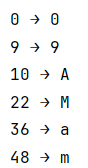
\includegraphics[height=2.5cm]{Bilder/Labelzuordnung}
				\caption{Zuordnung Label zu Buchstabe}
				\label{fig:labelzuordnung}
			\end{figure}

		\subsubsection{Datenbeschaffung}
			Für die gestellten Anforderungen an den Datensatz wurde die Klasse PerpareData geschaffen, die die zentrale Rolle bei der Aufbereitung und Balancierung der Datensätze für das Training und die Evaluation des Modells übernimmt. Ziel ist es, für jede Klasse eine festgelegte Anzahl an Beispielen im Trainings- und Testdatensatz bereitzustellen. 
			
			Die Klasse \texttt{PrepareData} erwartet als Eingabe den vordefinierten EMNIST Test- und Trainingsdatensatz, sowie die gewünschten numerischen Labels, die im Datensatz berücksichtigt werden sollen. Danach muss lediglich die Methode \textit{getData()} mit der gewünschten Parametrisierung aufgerufen werden, wie z.B. Anzahl der Klassen für Trainings- und Testdatensatz, ob ein Validierungsdatensatz von den Testdaten abgezogen oder wie mit zu wenigen Test- und Trainingsdaten umgegangen werden soll.
			
			Das Vorgehen der Methode \textit{getData()} lässt sich wie folgt zusammenfassen:
			\begin{enumerate}
				\item \textbf{Balancierung des Testdatensatzes} \\
				Zuerst wird überprüft, ob für jede Klasse im Testdatensatz genügend Beispiele (in unserem Fall 1000) vorhanden sind.
				\begin{itemize}
					\item \textbf{Zu viele Testbeispiele:} Sind ausreichend Beispiele vorhanden, wird eine zufällige Auswahl getroffen, sodass die gewünschte Anzahl von Testbeispielen nicht überschritten wird.
					\item \textbf{Zu wenige Testbeispiele:} Falls für eine Klasse zu wenige Testbeispiele existieren, werden die fehlenden Beispiele zufällig aus dem Trainingsdatensatz entnommen und dem Testdatensatz hinzugefügt. Diese Beispiele werden gleichzeitig aus dem Trainingsdatensatz entfernt, um Überschneidungen zu vermeiden.
				\end{itemize}
				
				Das Abziehen von Beispielen aus dem Trainingsdatensatz ist bei fehlenden Testdaten unerlässlich da im Gegensatz zum Trainingsdatensatz Testdaten nicht künstlich durch Augmentationen erweitert werden dürfen, weil dies die Aussagekraft der Modellbewertung verfälschen würde. Der Testdatensatz soll ausschließlich aus realen, im Datensatz vorhandenen Beispielen bestehen, um eine unverfälschte Evaluation des Modells zu ermöglichen. Gleichzeitig wird durch das Entfernen dieser Beispiele aus dem Trainingsdatensatz verhindert, dass identische Daten sowohl zum Training als auch zur Evaluation verwendet werden, was zu einer Überschätzung der Modellleistung führen könnte. Dadurch entsteht ein neuer, balancierter Testdatensatz und ein entsprechend reduzierter Trainingsdatensatz. Zusätzlich zur manuellen Überprüfung, bzgl. der Fehlerfreiheit des Codes, werden zur Nachvollziehung des Prozesses entsprechende Texte auf der Konsole ausgegeben. 
				\begin{lstlisting}[basicstyle=\small\ttfamily]
				Klasse B: Test 648 - Train 352
				Klasse C: Test 1000 - original Test 1739
				Klasse D: Test 779 - Train 221
				[...]
				Label H: Train 2673 augmentated 2327
				Trainingsdaten nach Label H: 90000
				Label I: Train 5000 orig 5000
				Trainingsdaten nach Label I: 95000
				\end{lstlisting}
			
			
				\item \textbf{Balancierung und Augmentation des Trainingsdatensatzes} \\
				Anschließend wird für die Trainingsdaten geprüft, ob die gewünschte Anzahl an Trainingsbeispielen von jeder Klasse erreicht wird.
				\begin{itemize}
					\item \textbf{Zu viele Trainingsbeispiele:} Sind ausreichend Beispiele vorhanden, wird eine zufällige Auswahl getroffen, sodass die gewünschte Anzahl von Trainingsbeispielen nicht überschritten wird.
					\item \textbf{Zu wenige Trainingsbeispiele:}  Falls für eine Klasse zu wenige Testbeispiele existieren, werden die fehlenden durch mehrfaches Hinzufügen der vorhandenen Beispiele ausgeglichen, wobei für diese ein Augmentierungs-Flag gesetzt wird. Dieses Flag signalisiert, dass auf Beispiele während des Trainings künstlich durch Datenaugmentation angereichert werden, um die Vielfalt der Daten zu erhöhen und um Overfitting, eine zu starke Anpassung des Modells an die Trainingsdaten zu vermeiden. Der Code garantiert, dass jedes Beispiel gleich oft für die Datenaugmentierung ausgewählt, falls mehr als die Hälfte der Beispiele mit Augmentierungen angereichert werden müssen.
				\end{itemize}
				
				
				\item \textbf{Abspalten des Validierungsdatensatzes aus dem Trainingsdatensatz} \\
				Wenn es der User wünscht, kann er sich von den Testdaten einen Validierungsdatensatz in gewünschter Größe abspalten lassen. Zum Validierungsdatensatz gibt es wie beim Testdatensatz ein Augmentierungsflag, dass bestimmt, ob das jeweilige Beispiel augmentiert werden muss. Im Gegensatz zum Testdatensatz darf der Validierungsdatensatz wieder Augmentierungen enthalten, wenn dies für Sinnvoll gehalten wird. Bzgl. mangelnder Beispiele im reinen Trainingsdatensatz in bestimmten Klassen wurde die mögliche Augmentierung des Validierungsdatensatzes in Kauf genommen, da ansonsten trotz Augmentierungen die Vielfalt der Trainingsdaten leiden könnte.
			
				\item \textbf{Überprüfung der Daten} \\
				Zur Überprüfung kann man mit einer Methode der Klasse \texttt{PerpareData} die Labels des Datensatzes nochmal manuell zählen, indem einzeln über die Beispiele mit ihren Labels iteriert wird. \\
	
			\end{enumerate}
			
			
			

			

			

			\textbf{Schwierigkeiten} \\
			Eine Herausforderung war es die Anzahl der Beispiele der einzelnen Klassen effizient zu zählen. Es hat sich bewährt auf den Ursprünglichen Datensatz immer wieder zurückzukehren, bzw. mit diesen zu arbeiten, indem Sub-Datensätze basierend auf den Originalen Datensatz erstellen werden, da dieser bereits eine Label Liste zu den einzelnen Beispielen enthält. Mit dieser kann anschließend eine Binäre Maske zu den jeweiligen Klassenlabel erzeugt werden, mit der effizient alle Beispiele aus den Original-Datensatz ausgewählt werden können. Mit einer Schleife durch alle Beispiele zu iterieren, um die Labels manuell zu zählen hat sich als uneffektiv herausgestellt.

			\textbf{Zusammenfassung} \\
			Das Vorgehen stellt sicher, dass sowohl Trainings- als auch Testdatensatz für jede Klasse eine festgelegte Anzahl an Beispielen enthalten. Fehlende Beispiele aus dem Testdatensatz werden aus dem Trainingsdatensatz ergänzt und im Trainingsdatensatz durch Augmentation künstlich erzeugt. Dadurch sollte eine ausgewogene und robuste Datenbasis für das Training und die Evaluation des Modells geschaffen sein.

		\subsubsection{Normierung und Skalierung des Datensatzes}
			Auch beinhaltet die Klasse \texttt{PrepareData} eine Methode, die vom ursprünglich gesamten Trainingsdatensatz den aktuellen durchschnittlichen Mittelwert, sowie die Standardabweichung aller Pixel aller Bilder ermittelt und zurückgibt. Diese wird in der Regel vor dem Balancieren des Datensatzes aufgerufen. Beim Laden des Datensatzes von der Bibliothek PyTorch wird die bereits eine Transformation der Bilder durchgeführt, indem diese auf den Bereich 0-1 skaliert und mit den aktuell ermittelten Mittelwert sowie der Standardabweichung dieser Methode normiert werden. Nach der Normierung beträgt der Mittelwert über alle Bilder 0 und die Standardabweichung 1. Die Normalisierung der Bilder trägt zur Besseren Leistungsfähigkeit des Modells statt. Der Testdatensatz muss später ebenfalls mit den ermittelten Werten aus den Trainingsdatensatz normiert werden, da das Modell mit diesen Normierungswerten trainiert worden ist.
			
			
			
			
			
	\subsection{Datenverarbeitung}
		\subsubsection{Label Mapping auf die Ausgänge des Neuronalen Netzes}
			Für die weitere Verarbeitung der Daten wurde eine eigene Dataset-Klasse \texttt{DatasetEMNIST} implementiert, die speziell auf die Anforderungen des Projekts zugeschnitten ist. Da für unsere Anforderungen nur ein Teil der EMNIST-Datensatz enthaltenen Klassen verwendet wird, muss ein Label-Mapping auf die Ausgänge des Neuronalen Netz durchgeführt werden.
			Die Klasse sorgt dafür, dass die \textbf{Labels der Zeichen-Klassen auf die 36 Ausgänge des Neuronalen Netzes, dass einen zusammenhängenden Bereich von 0 bis 35 erwartet zugeordnet werden}. Eine weitere Aufgabe der Klasse ist die gezielte Anwendung von Datenaugmentationen auf den Trainings- und Validierungsdaten, um die Vielfalt der Trainingsdaten zu erhöhen und das Modell robuster gegenüber Variationen zu machen. Wird eine Augmentierungs-Flag-Liste der Klasse übergeben, prüft diese bei jedem Beispiel, dass angefordert wird, ob eine Augmentierung angewandt werden soll. 
		
		\subsubsection{Anwendung von Augmentierungen}
			Für die Augmentierungen wurde ein \texttt{OneOf}-Sampler geschaffen, der für jedes Bild, das augmentiert werden soll, eine zufällige in der Klasse definierte Augmentierung ausgewählt und anwendet. Die Wahrscheinlichkeiten für die Auswahl der jeweiligen Transformation können dabei individuell angepasst werden und wurden später in der Hyperparameter-Optimierung als Parameter definiert und optimiert.
		
		\subsubsection{Auswahl der Datenaugmentierung}
			Um die Vielfalt der Trainingsdaten zu erhöhen und das Modell robuster gegenüber Eingaben zu machen, werden verschiedene Bildtransformationen eingesetzt. Diese wurden zuerst im Jupyter-Notebook \texttt{main.ipynb} \cite{noauthor_project_nodate} visualisiert und bewertet. Die Wahl fiel auf die Augmentationen GaussianBlur, RandomRotation sowie RandomResizedCrop. 
			Nachfolgend finden sie eine Übersicht der Auswirkungen der ausgewählten Augmentationen. Die Visualierungen dazu sind im  \hyperref[subsec:augmentation-visualization]{\textcolor{darkblue}{Anhang unter \ref*{subsec:augmentation-visualization} \nameref{subsec:augmentation-visualization}}} zu finden.
			
			\begin{itemize}
				\item \textbf{GaussianBlur} \\
					Das Bild wird mit dem Gaußschen Unschärfe bearbeitet. Dadurch werden feine Details und Kanten im Bild abgeschwächt, was das Modell dazu zwingt, robustere und allgemeinere Merkmale zu lernen, anstatt sich auf kleine Bilddetails zu verlassen.
				\item \textbf{RandomRotation} \\
					Das Bild wird um einen zufälligen Winkel innerhalb eines definierten Bereichs gedreht. Diese Transformation hilft dem Modell, robuster gegenüber unterschiedlichen Schreibrichtungen und leichten Verdrehungen der Zeichen zu werden. Der Grad der Rotation wurde von -15° bis 15° variable festgesetzt.
				\item \textbf{RandomResizedCrop} \\
					Aus dem Bild wird ein zufälliger Ausschnitt ausgewählt und anschließend auf die ursprüngliche Bildgröße (z.B. 28x28 Pixel) skaliert. Dadurch lernt das Modell, auch mit unterschiedlichen Positionen und Größen der Zeichen innerhalb des Bildes umzugehen und wird weniger empfindlich gegenüber Verschiebungen und Skalierungen. Der Zoomfaktor wurde auf eine variable Größe zwischen 80\,\% -- 100\,\% festgesetzt.
			\end{itemize}

		
			
			Auch wurden noch weitere Transformationen wie \texttt{RandomErasing}, oder \texttt{RandomAffine} für Affine Transformationen mit verschiedenen Parametrisierungen ausprobiert. Es wurde sich letztendlich dagegen entschieden, diese Augmentierungs-Methoden mit aufzunehmen, da mit \texttt{RandomResizedCrop} und \texttt{RandomRotation} die Transformationen von \texttt{RandomAffine} schon sehr gut abgedeckt wurden und der Effekt von \texttt{RandomErasing} auf unserer Bildgröße von 28x28 Pixeln das Bild zu sehr verunreinigt hat.

\section{Modellarchitektur}
	\subsection{Ursprüngliche Modellarchitektur}
		Für die Klassifikation der handgeschriebenen Zeichen wurde ein Transfer-Learning Ansatz mit einem vortrainierten ResNet-18 Modell \cite{he_deep_2015} verwendet, dass ursprünglich für die Bildklassifikation auf dem ImageNet-Datensatz \cite{noauthor_imagenet_nodate} mit RGB-Bildern entwickelt wurde. ResNet-18 ist ein Convolutional Neural Network, das bereits eine Vielzahl von Bildmerkmalen erlernt hat. Dadurch lässt sich die Trainingszeit, sowie der Datenbedarf erheblich reduzieren.
		Da der EMNIST-Datensatz Graustufenbilder mit nur einem Kanal enthält, wurde der erste Convolutional Layer des ResNet-18 ausgetauscht, sodass das Netz Eingabebilder mit nur einen Farbkanal verarbeiten kann. Darüber hinaus musste der finale Klassifikations-Layer (auch Fully Connected Layer genannt) des Modells auf unsere Anzahl von 36 Zeichen-Klassen angepasst werden.
	
	
	\subsection{Experimentelle Modellarchitektur}
		Im Rahmen der Projektarbeit sollte zusätzlich untersucht werden, ob die Leistung des Modells mit einem zweiten Klassifikator zusätzlich gesteigert werden kann. Dafür soll der unser Ansatz, um ein zweites Modell ergänzt werden, dass aber gemeinsam trainiert und optimiert werden soll. Der erste Klassifikator soll weiterhin die 36 Zeichen-Klassen und der zweite Klassifikator, ob es sich um einen Großbuchstaben, Kleinbuchstaben oder eine Ziffer handelt vorhersagen. Die Wahrscheinlichkeiten von beiden sollen miteinander multipliziert werden und bilden einen neuen zusammengesetzten Klassifikator. Das Ziel war es Fehler zwischen ähnlichen Klassen, wie z.B. zwischen Groß- und Kleinbuchstaben (c/C) zu reduzieren.
		Es wurden zwei verschiedene Ansätze umgesetzt.
	
		\subsubsection{Experimentelle Modellarchitektur - Ansatz 1}
			Die Klasse \texttt{CombinedClassifier} kombiniert zwei Modelle innerhalb einer gemeinsamen Architektur: 
			\begin{itemize}
				\item \textbf{Teilmodul 1} 
					ist der ursprüngliche Klassifikator, der wie bisher die 36 feingranularen Klassen (Ziffern, Groß- und Kleinbuchstaben) unterscheidet. 
				\item \textbf{Teilmodul 2}
					stellt einen zusätzliches kompaktes CNN-Netzwerk dar, dass lediglich zwischen den drei Oberklassen (Großbuchstabe, Kleinbuchstabe, Ziffer) unterscheidet.
			\end{itemize}

			Für die Vorhersage werden beide Modelle parallel auf das Eingabebild angewendet. Für jede Klasse berechnet das erste Modell die Wahrscheinlichkeiten für alle 36 Zeichenklassen, während das zweite Modell die Wahrscheinlichkeit für die jeweilige Oberklasse liefert. Die Wahrscheinlichkeiten der 36 Zeichenklassen wird anschließend mit seiner jeweiligen Oberklasse multipliziert und final zurückgegeben.
			
			Teilmodul 2 besteht aus drei aufeinanderfolgenden Convolution-Blöcken mit Batch\-Norm-, ReLU{-}, und Max\-Pool-Schichten, gefolgt von mehreren voll verbundenen Linear-Layern mit Dropout und ReLU-Aktivierungsfunktion.

			\begin{lstlisting}[language=Python, basicstyle=\small\ttfamily]
self.tm2 = nn.Sequential(
	# Block 1 - Shape after Conv2d: (16, 28, 28)
	nn.Conv2d(1, config['conv2d_out_1'], kernel_size=config['conv2d_kernel_size_1'], stride=1, padding=padding1),  
	nn.BatchNorm2d(config['conv2d_out_1']),
	nn.ReLU(),
	nn.MaxPool2d(2),  # (16, 14, 14)
	
	# Block 2 - Shape after Conv2d: (32, 14, 14)
	nn.Conv2d(config['conv2d_out_1'], config['conv2d_out_2'], kernel_size=config['conv2d_kernel_size_2'], stride=1, padding=padding2),  
	nn.BatchNorm2d(config['conv2d_out_2']),
	nn.ReLU(),
	
	# Block 3 - Shape after Conv2d: (32, 14, 14)
	nn.Conv2d(config['conv2d_out_2'], config['conv2d_out_3'], kernel_size=config['conv2d_kernel_size_3'], stride=1, padding=padding3),  # 
	nn.BatchNorm2d(config['conv2d_out_3']),
	nn.ReLU(),
	nn.MaxPool2d(2),  # (64, 7, 7)
	
	nn.Flatten(),
	nn.Linear(config['conv2d_out_3'] * 7 * 7, config['linear_out_1']),
	nn.Dropout(config['dropout']),
	nn.ReLU(),
	nn.Linear(config['linear_out_1'], config['linear_out_2']),
	nn.ReLU(),
	nn.Linear(config['linear_out_2'], num_out_classes_tm2)  # 3 Klassen
)
			\end{lstlisting}
			
			Die \texttt{config}-Parameter der einzelnen Schichten in Teilmodul 2 wurden für die Hyper\-parameter-Optimierung als Variable Parameter definiert, die beim Initialisieren der Klasse übergeben werden.
		
		\subsubsection{Experimentelle Modellarchitektur - Ansatz 2}
			Anstatt zwei separate neuronale Netze für die Bildverarbeitung zu verwenden, arbeitet die Klasse \texttt{CombinedClassifier2} mit nur einen Neuronalen Netz, nutzt aber zwei verschiedene Classification Layer am Ende des Netzes. Die Classification Layer nutzen also die gleichen Eingabefeatures. 
			\begin{itemize}
				\item \textbf{Classification Layer 1} 
				ist weiterhin ein Linear-Layer, der die 36 feingranularen Zeichenklassen (Ziffern, Groß- und Kleinbuchstaben) unterscheidet.
				\item \textbf{Classification Layer 2}
				besteht aus einen mehrschichtigen kompakten Neuronalen Netzwerk das die 3 Oberklassen Ziffer, Klein- / Großbuchstabe klassifiziert.
			\end{itemize}
			
			Die Multiplikation beider Classification Layer erfolgt identisch wie in Ansatz 1 beschrieben.
			
			Für den Classification Layer 2 wurden 3 Linear-Layer mit der ReLU-Aktivierungsfunktion ausgewählt, mit zusätzlichen Dropout-Layer nach dem ersten Linear-Layer um dem Overfitting des Classification Layers entgegenzuwirken.
			\begin{lstlisting}[language=Python, basicstyle=\small\ttfamily]
# TM1: CNN mit 36 Klassen
self.tm1 = nn.Linear(in_features_tm, num_out_classes_tm1)

# TM2: Neues Modul
self.tm2 = nn.Sequential(
	nn.Linear(in_features_tm, config['linear_out_1']),
	nn.Dropout(config['dropout']),
	nn.ReLU(),
	nn.Linear(config['linear_out_1'], config['linear_out_2']),
	nn.ReLU(),
	nn.Linear(config['linear_out_2'], num_out_classes_tm2)
)
			\end{lstlisting}
			Die Anzahl der Ein- und Ausgabe Features der einzelnen Schichten, sowie die Wahrscheinlichkeit mit der im Dropout-Layer einzelne Neuronen deaktiviert werden, wurden für die Hyperparameter-Optimierung als Variable Parameter definiert.
			
			
		
\section{Trainingsprozess}
	Für das Modelltraining wurde die Klasse EMNISTModel erstellt, die die Trainings- Validierungs- und Testphasen eines Modelltrainings automatisch regelt. 
	
	Die Klasse erwartet einen Experiment-Namen, um z.B. die Modell-Logging-Pfade zu vervollständigen. Auch ob im Trainingsprozess nach jeder Epoche eine Validierung durchgeführt werden soll, kann hier festgelegt werden. 
	
	Wird die \textit{test()}-Methode der Klasse \texttt{EMNISTModel} aufgerufen wird automatisch der EMNIST Datensatz geladen und das Modelltraining gestartet. Beim Laden des EMNIST Datensatzes wird eine Skalierung auf 0-1 und anschließend eine Normierung anhand der Standardabweichung und des Mittelwertes vom ursprünglichen gesamten vordefinierten EMNIST Trainingsdatensatz auf unseren geladenen Daten durchgeführt. 
	Die Klasse \texttt{PrepareData} gibt uns anschließend den Test-, Trainings- und Validierungsdatensatz mit ihren Augmentierungs-Flag-Listen zurück, die als Eingabe unserer angepassten \texttt{EMNISTDataset}-Klasse dienen. Diese managt, wie schon beschrieben die Augmentierungen und das Label-Mapping für unser Netzwerk. Anschließend werden die jeweiligen \texttt{Dataloader} mit der übergebenen Batch-Größe initialisiert und das Modelltraining gestartet.
	
	\subsection{Trainingsstrategie}
	  Das Training des Modells erfolgt in Mini-Batches, da dies eine schnellere Konvergenz des Modells gewährleistet, wenn nur mit Batches über den gesamten Trainingsdatensatz gearbeitet wird. Wie typisch bei Klassifikationsaufgaben mit mehreren Klassen wird die Cross-Entropie-Verlustfunktion \cite{noauthor_crossentropyloss_nodate} verwendet. Diese erwartet die Logits (Rohwerte) des Modells und wendet intern eine Softmax-Aktivierungsfunktion an, um die Klassenwahrscheinlichkeiten zu erhalten. Die Verlustfunktion dient dazu, den grad der Abweichung der Vorhersage zum wahren Wert zu bestimmen. 
	  
	  Als Optimizer kommt der \texttt{AdamW}-Optimizer zum Einsatz, der sich durch eine adaptive Lernratenanpassung und Gewichtsnormierung auszeichnet und ist maßgeblich daran beteiligt, wie das Netzwerk sich optimiert. Der \texttt{AdamW}-Optimizer soll gegenüber des ursprünglichen Adam-Optimizers \cite{noauthor_adam_nodate} zu stabilerer Konvergenz und besserer Generalisierung führen. Zusätzlich wird ein \texttt{ReduceLROnPlateau}-Scheduler \cite{noauthor_reducelronplateau_nodate} verwendet, der die Lernrate automatisch reduziert, sobald sich die Validierungsleistung über mehrere Epochen nicht verbessert. Dadurch wird das Modell vor Überanpassung geschützt und kann auch in späteren Trainingsphasen noch weiter lernen. Da wir den \texttt{ReduceLROnPlateau}-Schuduler benutzen, bedeutet es gleichzeitig, dass immer ein Validierungsdatensatz für das Modelltraining benötigt wird.
	  
	  Nach jeder Epoche wird die Modelleistung mit den Validierungsdatensatz gemessen und den Scheduler für seine Optimierungsmaßnahmen übergeben.
	  
	  Die \textit{train()}-Methode erwartet die Parameter zum Scheduler, Optimizer, sowie die Lernrate, Batch-Größe und Anzahl der Epochen, ob nur der Classifikation-Layer trainiert und ob der \texttt{CombinedClassifier}/\texttt{CombinedClassifier2} zum Einsatz kommen soll und wiederum dessen Parameter als Hyperparameter. 
  
  
  
  	\subsection{Evaluation und Protokollierung}

		 
		 \subsubsection{Messung der Modellleistung}
		 Die Modellleistung wird, sowohl beim Testen als auch beim Validieren anhand folgender Metriken gemessen:	 
		 \begin{table}[h]
		 	\centering
		 	\begin{tabular}{|l|>{\raggedright\arraybackslash}m{0.7\linewidth}|}
		 		\hline
		 		\rowcolor{lightgray} \multicolumn{1}{|c|}{\textbf{Metrik}} & \multicolumn{1}{c|}{\textbf{Bedeutung}} \\
		 		\hline
		 		\verb|Top-1 Accuracy| & Prozentualer Anteil, wie oft Vorhersage des Modells richtig war \\
		 		\hline
		 		\verb|Top-3 Accuracy| & Prozentualer Anteil, wie oft die richtige Vorhersage in den Top-3 Vorhersagen des Modells war \\
		 		\hline
		 		\verb|Top-3 Accuracy| & Prozentualer Anteil, wie oft die richtige Vorhersage in den Top-5 Vorhersagen des Modells war \\
		 		\hline
		 		\verb|Loss| & Durchschnittlicher Loss aller Evaluierungs-Vorhersagen \\
		 		\hline
		 	\end{tabular}
		 	\caption{Metriken zur Messung der Leistung des Modells}
		 	\label{tab:Metriken}
		 \end{table}
		 	 
		 Nach dem Modelltraining kann die Methode \textit{test()} der \texttt{EMNISTModell}-Klasse aufgerufen werden, um die Leistung des Modells auf den zuvor ermittelten Test-Datensatz zu Evaluieren. Im Anschluss werden die Metriken des Ergebnisses der Evaluierung in die Konsole gedruckt, als auch eine Confusion-Matrix als Bild zum Experiment-Namen gespeichert. Anhand der Confusion-Matrix kann abgelesen werden, welche Zeichen zu welcher Klasse vorhergesagt wurden und wo schwächen im Modell liegen.
		 Das Modelltraining kann nicht nur direkt nach dem Modelltraining, sondern auch separat gestartet werden indem der Checkpoint-Pfad zum gespeicherten Modell übergeben wird. Um die gleichen unabhängigen Testdaten wie bei der Dateninitialisierung beim Training zu erhalten wurde ein Seed für die \textit{random()}-Methode gesetzt, der gleichen Output Trainings-Test-Split garantiert.
		 
		 
   		\subsubsection{Protokollierung}
		 Während des Trainings können wichtige Metriken, sowie der Loss regelmäßig geloggt werden. Hierfür gibt es eine eigene Logging-Klasse \texttt{ModelLogging}, die sowohl die Speicherung von Checkpoints als auch die Integration mit TensorBoard \cite{noauthor_tensorboard_nodate} unterstützt. Die Klasse \texttt{ModelLogging} greift wiederum auf Methoden der Klasse \texttt{LoggingTB} (für TB = TensorBoard) und \texttt{ModelPersistence} (für Checkpoints) zurück. Wurde das Logging der \textit{train()}-Methode aktiviert, wird der alle 10 Batches der Loss, sowie nach jeder Epoche die Modellleistung in TensorBoard protokolliert. Zusätzlich merkt sich das Programm die Beste Modellleistung bzgl. aller Modellleistungs-Metriken und zeichnet diese zusätzlich auf, wenn sich die jeweilige Metrik verbessert hat. So kann man bei der Auswertung den Trend des Modells erkennen, in welchen Epochen eine bessere Modellleistung erzielt wurde. Am Ende des Trainings wird das Modell mitsamt seinen Parametern in einer \texttt{.pth}-Datei abgespeichert, um es nach dem Training weiterhin nutzen zu können.
		 
		 
		 \textbf{In TensorBoard werden während des Trainings folgende Werte aufgezeichnet:}
		 \begin{figure}[h!]
		 	\centering
		 	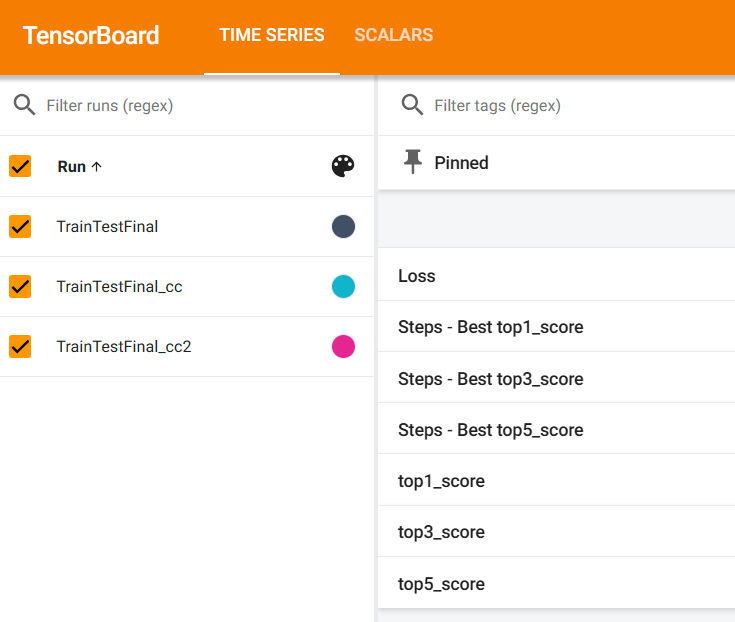
\includegraphics[width=0.6\linewidth]{Bilder/TB_3.png}
		 	\caption[Aufgezeichnete Werte in TensorBoard]{Aufgezeichnete Werte in TensorBoard}
		 	\label{fig:TB3}
		 \end{figure}
		 
		 Dabei wird nach jeder Validierung die Top-1, Top-3 und Top-5 Accuracy aufgezeichnet sowie immer in welcher Epoche sich die jeweilige Accuracy verbesserte (siehe \texttt{Steps-Best top5\_score})
  
  
  \section{Hyperparameter-Tuning}
  Beim Hyperparamater-Tuning wird versucht die Modellparameter für die Beste Leistung des Modells zu finden. Als Hyperparameter-Tuning Framework wurde OPTUNA \cite{noauthor_optuna_nodate} eingesetzt. OPTUNA ermöglicht einfaches Hyperparameter-Tuning, indem Suchräume jeden Hyperparameter definiert werden können. Für die einfachere Handhabung wurde die Klasse HyperparameterTuning erstellt, das Methoden für das Hyperparameter-Tuning und die Auswertung der Ergebnisse enthält. So können auch von einem durchgeführten Tuning die Besten 10 ermittelten Konfigurationen ausgegeben werden.
  Für das Tuning wurde der \texttt{MedianPruner} ausgewählt, der beim Tuning die zu schlechten Konfigurationen stoppt und mit der nächsten fortfährt. Nach den ersten 3 Epochen misst er die Leistung des Modells anhand der Top-1 Accuracy und bricht das Training ab, wenn diese unter dem Median aller bisherigen Top-1 Accuracy der bisherigen Konfigurationen liegt. Anschließend wird in regelmäßigen Abständen von jeweils drei Intervallen geprüft, ob eine Konfiguration fortgesetzt oder abgebrochen werden soll, um den Einfluss temporärer Leistungsschwankungen zu minimieren.
  
  
  \section{Durchführung des Hyperparameter-Tunings und Auswahl des besten Modells}	  

	  \begin{table}[h]
	  	\centering
	  	\begin{tabular}{|>{\raggedright\arraybackslash}m{0.4\linewidth}|>{\raggedright\arraybackslash}m{0.55\linewidth}|}
	  		\hline
	  		\rowcolor{lightgray} \multicolumn{1}{|c|}{\textbf{Was}} & \multicolumn{1}{c|}{\textbf{Speicherort „Logging/…“}} \\
	  		\hline
	  		\multicolumn{2}{|l|}{\small\rule{0pt}{1.5em}\textbf{Logging Hyperparameter-Tuning}} \\ 
	  		\hline
	  		10 Besten Hyperparameter-Konfigurationen & \scalebox{0.9}{\mbox{Optuna/Ergebnisse HT/Auswertung\_Top10\_HT.txt}} \\ 
	  		\hline
	  		Details und Ergebnisse zu allen Hyperparameter-Konfigurationen & \scalebox{0.9}{\mbox{Optuna/Ergebnisse HT/ConsoleOutputHT.txt}} \\ \hline
	  		Ergebnis-Datenbank Optuna & \scalebox{0.9}{\mbox{Optuna/optuna\_HT.db}} \\ 
	  		\hline
	  		\multicolumn{2}{|l|}{\small\rule{0pt}{1.5em}\textbf{Logging Finales Modell - Ergebnisse auf dem Testdatensatz}} \\ 
	  		\hline
	  		Details zum Trainingsprozess bzgl. des Validierungsdatensatzes & \scalebox{0.9}{\mbox{TensorBoard/TrainTestFinal/}} \\ 
	  		\hline
	  		Trainings-Details und Test-Ergebnis & \scalebox{0.9}{\mbox{ConsoleOutput/output\_TrainTestFinal.txt}} \\ 
	  		\hline
	  		Confusion Matrix & \scalebox{0.9}{\mbox{ConfusionMatrix/TrainTestFinal.png}} \\ 
	  		\hline
	  	\end{tabular}
	  	\caption{Datei-Logging-Speicherorte des Modells mit eigenen Classifier}
	  	\label{tab:Speicherorte}
	  \end{table}
	  
	  Ursprünglich wurde das ResNet-18 Model auf den ImageNet-Datensatz mit RGB-Bildern trainiert. Im Umkehrschluss heißt das, dass die vortrainierten Gewichte auf RGB-Bilder mit einer Größe von 224x224 abgestimmt sind. In den ersten Experimenten wurden die Bilder aus dem EMNIST Datensatz auf 224x224 hochskaliert und die Farbkanal-Dimension verdreifacht. Es stellte sich jedoch später durch das Hyperparameter-Tuning heraus, dass dies fast keinen Mehrwert brachte, jedoch das Training sich um den Faktor 6 verlängerte. Anschließend wurde nur noch mit der ursprünglichen Bildgröße 28x28 weitergearbeitet.
	  	  
	  Im Logging Ordner des Projekts können alle relevanten Dateien gefunden werden, um das nachfolgende Hyperparameter Tuning nachzuvollziehen.
  
  
  
  
  
  %###############################
  \subsection{Modell Resnet-18 mit eigenen Classifier}

	Die \textbf{Speicherorte der Logging-Dateien} liegen wie in \hyperref[tab:Speicherorte]{\textcolor{darkblue}{Tabelle \ref*{tab:Speicherorte}}} beschrieben unter den angegeben Pfaden.


\subsubsection{Hyperparameter-Tuning}
  Der Suchraum der Hyperparameter wurde zu Beginn nach kleiner Recherche wie folgt festgelegt:
\begin{lstlisting}[language=Python, basicstyle=\small\ttfamily]
	config = {
		"lr": trial.suggest_float("lr", 1e-5, 1e-2, log=True),
		"weight_decay": trial.suggest_float("weight_decay", 0.0001, 0.01, log=True),
		"num_epochs": trial.suggest_int("num_epochs", 12, 35),
		"batch_size": trial.suggest_categorical("batch_size", [16, 32, 64]),
		"only_train_classifier": trial.suggest_categorical("only_train_classifier", [True, False]),
		"sched_patience": trial.suggest_int("sched_patience", 2, 15),
		"sched_factor": trial.suggest_float("sched_factor", 0.1, 0.9),
		"sched_min_lr": trial.suggest_categorical("sched_min_lr", [1e-5, 1e-6]),
		'train_with_CombinedClassifier': False,
		'probabilities': [trial.suggest_float("a1", 0.1, 1), trial.suggest_float("a2", 0.1, 1), trial.suggest_float("a3", 0.1, 1), trial.suggest_float("a4", 0.1, 1)],
		'config_CombinedClassifier': None
	}
\end{lstlisting}
Die Bedeutung der Hyperparameter ist im Anhang \hyperref[tab:BedeutungHyperparameter]{\textcolor{darkblue}{Tabelle \ref*{tab:BedeutungHyperparameter}}} zu finden

	Insgesamt wurden im finalen Hyperparameter Tuning 40 verschiedene Kombinationen durchprobiert. Die Besten 10 Konfigurationen haben auf den Validierungsdatensatz alle eine Genauigkeit von ca. 90\,\% Top-1-Accuracy. Nachdem ich die Beste Konfiguration auf den Testdatensatz bewertete fiel die Top-1-Accuracy von 90,0\,\% auf ca. 82,0\,\% ab. Die Drastische Verschlechterung deutete auf Overfitting des Modells hin. Nach Untersuchung der Ergebnisse des Hyperparameter-Tunings konnte ich keine großartigen Verbesserungen nach einer bestimmten Epochenanzahl feststellen, weswegen ein Experiment mit den gleichen Konfigurationen, aber verringerter Epochenanzahl durchgeführt wurde. Auffallend ist zugleich, dass mit zunehmender Epochenanzahl die Top-3, bzw. die Top-5 Accurcy bei jeden meiner drei Modellarchitekturen wieder abfällt. Die Blaue Kurve stellt dabei das Modell mit der Epochenanzahl 25 dar, die Rote Kurve die Epochenanzahl 20, siehe \hyperref[fig:TensorBoardAccuracy]{\textcolor{darkblue}{Abbildung \ref*{fig:TensorBoardAccuracy}}}.

	\begin{figure}[h]
		\centering
		\subfigure[TensorBoard - Top-1 Accuracy]{%
			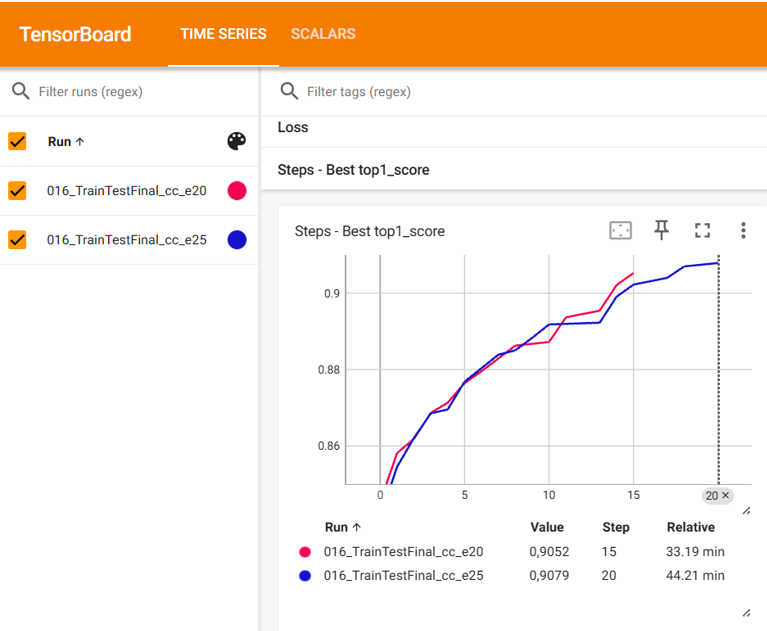
\includegraphics[width=7cm]{./Bilder/TB_1.png}
			\label{fig:TB1}
		}
		\hspace{0.5cm}
		\subfigure[TensorBoard - Top-3 Accuracy]{%
			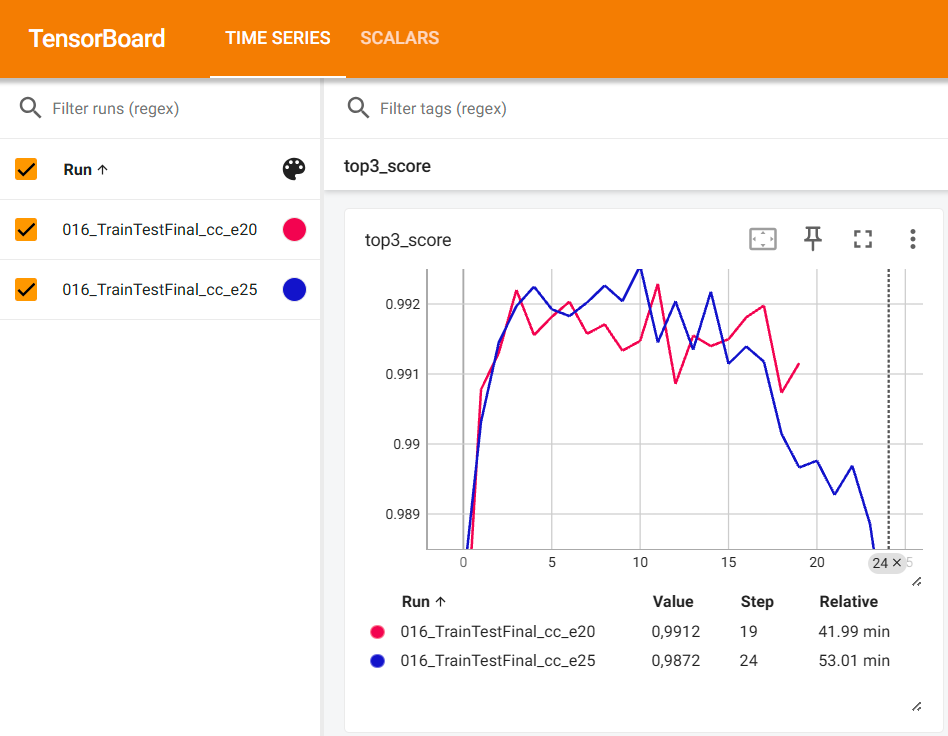
\includegraphics[width=7cm]{./Bilder/TB_2.png}
			\label{fig:TB2}
		}
		\caption{TensorBoard - Auswertung der Accuracy bzgl. Epochen}
		\label{fig:TensorBoardAccuracy}
	\end{figure}
	
	Die Genauigkeit konnte durch Verringerung der Epochenanzahl anschließend noch auf das Finale Ergebnis von 83,4\,\% gesteigert werden. Die Vermutung liegt nahe, dass der Validierungsdatensatz den Testdatensatz zu stark ähnelt und der Test-Datensatz viele Zeichen, die sich zum Verwechseln ähnlich sind, enthält. 
	
	Außerdem stellte sich beim Hyperparameter-Tuning heraus, dass verschiedene Konfigurationen ähnliche Leistungen erreichen. Beispielsweise hat der Hyperparameter \texttt{probabilities} für die Augmentations-Wahrscheinlichkeiten nur einen geringen Einfluss auf die Leistung des Modells, im Gegensatz zu \texttt{only\_train\_classifier}, der angibt ob alle Gewichte des Modells optimiert werden sollen, sollte für die beste Leistung auf \texttt{False} belassen werden.
	
  
  \subsubsection{Finales Modell}
  Folgende Parameterisierung hat sich für das finale Modell als günstig erwiesen:
  \begin{lstlisting}[language=Python, basicstyle=\small\ttfamily]
	config = {
		"lr": 0.000203,
		"weight_decay": 0.000205,
		"num_epochs": 16,
		"batch_size": 64,
		"only_train_classifier": False,
		"sched_patience": 5,
		"sched_factor": 0.442897,
		"sched_min_lr": 0.000001,
		'train_with_CombinedClassifier': False,
		'probabilities': [0.16, 0.51, 0.64],
		'config_CombinedClassifier': None
	}
  \end{lstlisting}
  
  
  \begin{table}[h!]
  	\centering
  	\begin{tabular}{|l|c|c|}
  		\hline
  		\rowcolor{lightgray} \textbf{Metrik} & \textbf{Ergebnis Validierungsdaten} & \textbf{Ergebnis Testdaten} \\ \hline
  		Top-1 Accuracy & 89,6\,\% & 83,4\,\% \\ \hline
  		Top-3 Accuracy & 99,2\,\% & 98,7\,\% \\ \hline
  		Top-5 Accuracy & 99,8\,\% & 99,6\,\% \\ \hline
  		Avg-Loss pro Bild & - & 0,717 \\ \hline
  	\end{tabular}
  	\caption{Ergebnisse des Finalen Modells}
  \end{table}
  
  
  Als Ergebnis erhielten wie oben schon beschrieben 83,4\,\% der Top-1-Accuracy. \\
  Anschließend wurde die Confusion Matrix ausgewertet um den Modellfehler genauer zu untersuchen. Die Confusion Matrix zeigt auf, bei welchen Bildern das Modell welche vorhersagen liefert und wie oft. Auf der vertikalen Achse ist die wahre Klasse des Bildes aufgetragen und auf der horizontalen Achse die vorhergesagte Klasse des Modells.
  Die Auswertung der Confusion Matrix zeigt, dass das Modell z.B. schwächen hat, die Zahl 1, i, I, l (Eins, kleines i, großes i, kleines L) oder ein c von einem C zu unterscheiden. So wurden beispielsweise 239-mal ein c für ein C und 542-mal ein C für ein c fälschlicherweise vorhergesagt, siehe \hyperref[fig:ConfusionMatrixTrainTestFinal]{\textcolor{darkblue}{Abbildung \ref*{fig:ConfusionMatrixTrainTestFinal}}}. Aufgrund der Fehler die vor allem bei leicht zu verwechselnden Buchstaben auftraten und der Tatsache, dass das Modell keinen Kontext zu anderen Buchstaben / Wörtern bei einer Vorhersage hat, ist das Ergebnis akzeptabel.
  
  
  \begin{figure}[h!]
  	\centering
  	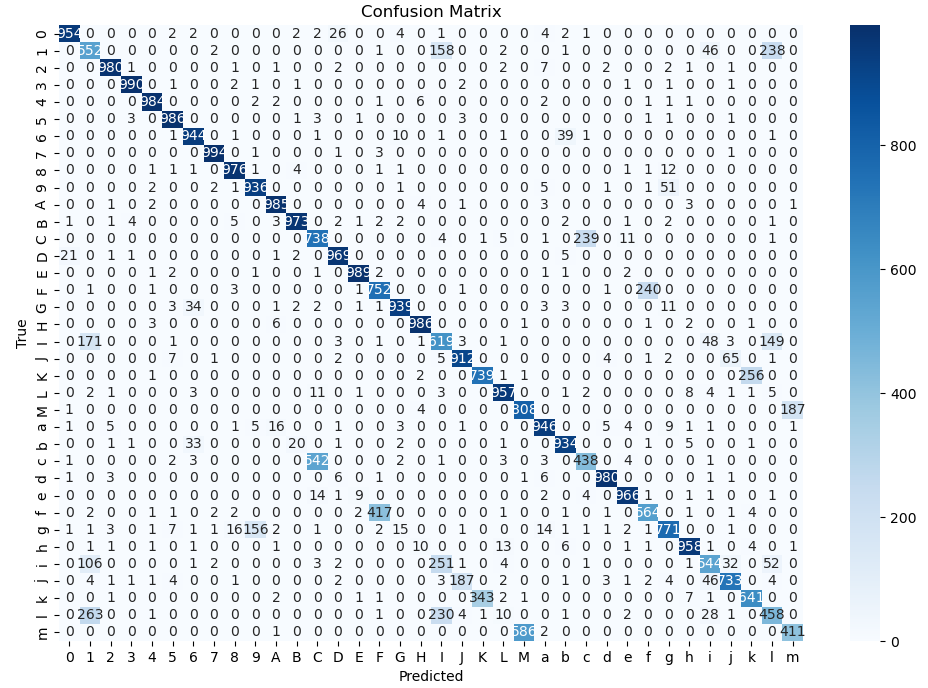
\includegraphics[width=0.9\linewidth]{Bilder/ConfusionMatrix/TrainTestFinal}
  	\caption[Confusion Matrix - Finales ursprüngliches Modell]{Confusion Matrix - Finales ursprüngliches Modell}
  	\label{fig:ConfusionMatrixTrainTestFinal}
  \end{figure}
  
  
  
  
  	%##############################
	\subsection{Modell Resnet-18 mit Experimentellen Classifier - Ansatz 1}
		Die \textbf{Speicherorte der Logging-Dateien} liegen wie in \hyperref[tab:Speicherorte]{\textcolor{darkblue}{Tabelle \ref*{tab:Speicherorte}}} beschrieben unter den angegeben Pfaden. Die Pfade ergänzen sich lediglich um den Zusatz „\_cc“ vor der Dateiendung.
		\subsubsection{Hyperparameter-Tuning}
	
			Der Suchraum der Hyperparameter wurde nach einer kleinen Internet-Recherche und den Erkenntnissen des ersten Hyperparameter-Tunings wie folgt festgelegt:
\begin{lstlisting}[language=Python, basicstyle=\small\ttfamily]
	config_CombinedClassifier = {
	'conv2d_out_1': trial.suggest_categorical("conv2d_out_1", [32, 64]),
	'conv2d_kernel_size_1': trial.suggest_categorical("conv2d_kernel_size_1", [3, 5]),
	'conv2d_out_2': trial.suggest_categorical("conv2d_out_2", [32, 64]),
	'conv2d_kernel_size_2': trial.suggest_categorical("conv2d_kernel_size_2", [3, 5]),
	'conv2d_out_3': trial.suggest_categorical("conv2d_out_3", [32, 64, 128]),
	'conv2d_kernel_size_3': trial.suggest_categorical("conv2d_kernel_size_3", [3, 5]),
	'linear_out_1': trial.suggest_categorical("linear_out_1", [128, 256, 512]),
	'linear_out_2': trial.suggest_categorical("linear_out_2", [32, 64, 128]),
	'dropout': trial.suggest_float("dropout", 0.1, 0.4),
}
config = {
	"lr": trial.suggest_float("lr", 1e-5, 1e-2, log=True),
	"weight_decay": trial.suggest_float("weight_decay", 0.0002, 0.01, log=True),
	"num_epochs": 25,
	"batch_size": trial.suggest_categorical("batch_size", [32, 64]),
	"only_train_classifier": False,
	"sched_patience": 5,
	"sched_factor": trial.suggest_float("sched_factor", 0.4, 0.7),
	"sched_min_lr": 1e-6,
	'train_with_CombinedClassifier': True,
	'probabilities': [0.5, 1, 1],
	'config_CombinedClassifier': config_CombinedClassifier
	}
\end{lstlisting}

	Die Epochenanzahl wurde auf 25 festgesetzt, weil die Epochenanzahl unnötig den Suchraum vergrößern würde und die Epochenanzahl eine gute Ausgangsbasis bildet, da das vorherige Modell oftmals nach 15-20 Epochen keine großen Verbesserungen mehr zeigte und wie schon zuvor beschrieben unter Overfitting leidete. Auch wurden durch den geringen Einfluss der Paramater \texttt{probabilities} auf einem festen Wert gesetzt und bewährte Hyperparameterwerte aus den Erfahrungen des vorherigen Tunings übernommen.
	

			\subsubsection{Finales Modell}
		    	Folgende Parameterisierung hat sich für das finale Modell als günstig erwiesen:
\begin{lstlisting}[language=Python, basicstyle=\small\ttfamily]
config_CombinedClassifier = {
	'conv2d_out_1': 32,
	'conv2d_kernel_size_1': 5,
	'conv2d_out_2': 64,
	'conv2d_kernel_size_2': 3,
	'conv2d_out_3': 64,
	'conv2d_kernel_size_3': 3,
	'linear_out_1': 128,
	'linear_out_2': 32,
	'dropout': 0.20,
}
config = {
	"lr": 3.825472731975857e-05,
	"weight_decay": 0.000469,
	"num_epochs": 25,
	"batch_size": 32,
	"only_train_classifier": False,
	"sched_patience": 5,
	"sched_factor": 0.442897,
	"sched_min_lr": 0.000001,
	'train_with_CombinedClassifier': True,
	'probabilities': [0.5, 1, 1],
	'config_CombinedClassifier': config_CombinedClassifier
}
\end{lstlisting}

Die Ergebnisse waren nach mehreren Durchläufen wie folgt:
  \begin{table}[h!]
	\centering
	\begin{tabular}{|l|c|c|}
		\hline
		\rowcolor{lightgray} \textbf{Metrik} & \textbf{Ergebnis Validierungsdaten} & \textbf{Ergebnis Testdaten} \\ \hline
		Top-1-Accuracy & 82,8\,\% & 83,0\,\% \\ \hline
		Top-3-Accuracy & 85,2\,\% & 84,2\,\% \\ \hline
		Top-5-Accuracy & 85,6\,\% & 84,5\,\% \\ \hline
		Avg-Loss pro Bild & - & 2,97 \\ \hline
	\end{tabular}
	\caption{Ergebnisse des Finalen Experimentellen Modells - Ansatz 1}
\end{table}


	
	Auffallend ist der sehr hohe Avg-Loss gegenüber den ursprünglichen Ansatz. Das Modell hat aber weiterhin die gleiche Top-1 Accuracy Leistung erzielt, ist dennoch wegen abfallender Top-3 Accuracy als schlechter zu bewerten. Es muss hier aber Erwähnt werden, dass bei gleicher Parameterisierung die Trainings- und Testergebnisse sehr schwanken können. Das könnte mehrere Ursachen haben, wie z.B. die implizite zufällige Initialisierung der Modellgewichte zu Beginn des Trainings, die sich als ungünstig erweisen könnte.
	
	Die Confusion Matrix zu den Ergebnissen ist in \hyperref[fig:ConfusionMatrixTrainTestFinalcc]{\textcolor{darkblue}{Abbildung \ref*{fig:ConfusionMatrixTrainTestFinalcc}}} zu sehen. 

  	
  \begin{figure}[h!]
  	\centering
  	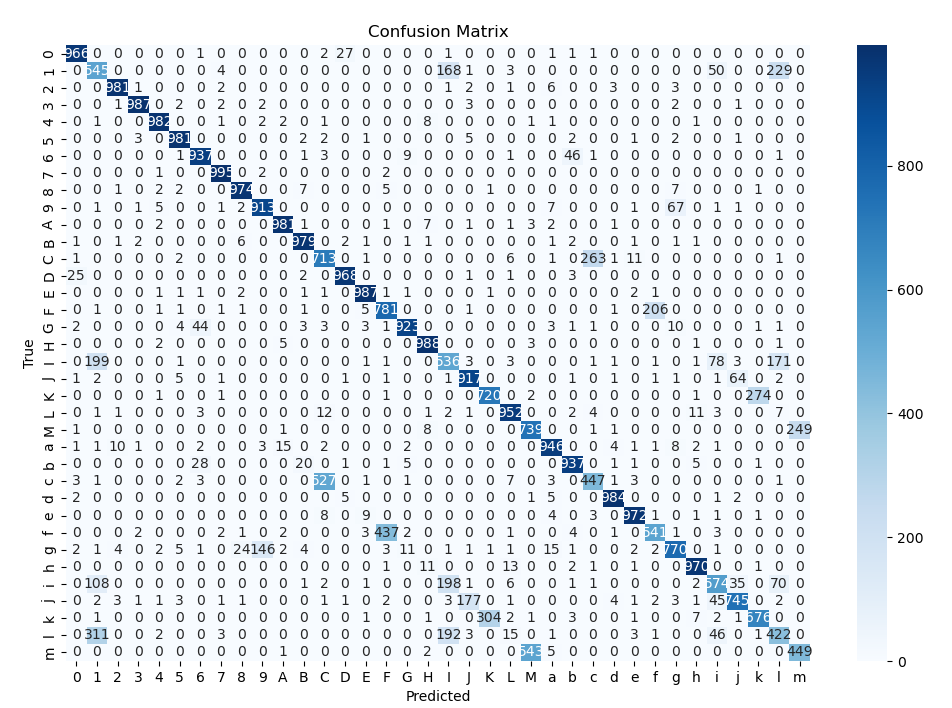
\includegraphics[width=0.8\linewidth]{Bilder/ConfusionMatrix/TrainTestFinal_cc}
  	\caption[Confusion Matrix des finalen experimentellen Modells - Ansatz 1]{Confusion Matrix - Finales experimentelles Modell - Ansatz 1}
  	\label{fig:ConfusionMatrixTrainTestFinalcc}
  \end{figure}
  
  
  %###############################
  \subsection{Modell Resnet-18 mit Experimentellen Classifier - Ansatz 2}
		Die \textbf{Speicherorte der Logging-Dateien} liegen wie in \hyperref[tab:Speicherorte]{\textcolor{darkblue}{Tabelle \ref*{tab:Speicherorte}}} beschrieben unter den angegeben Pfaden. Die Pfade ergänzen sich lediglich um den Zusatz „\_cc2“ vor der Dateiendung.
		
		
		\subsubsection{Hyperparameter-Tuning}
			Der Suchraum der Hyperparameter wurde nach einer kleinen Internet-Recherche und den Erkenntnissen des ersten Hyperparameter-Tunings wie folgt festgelegt:
\begin{lstlisting}[language=Python, basicstyle=\small\ttfamily]
config_CombinedClassifier = {
	'linear_out_1': trial.suggest_categorical("linear_out_1", [128, 256, 512]),
	'linear_out_2': trial.suggest_categorical("linear_out_2", [64, 128, 256]),
	'dropout': trial.suggest_float("dropout", 0.0, 0.4)
}
config = {
	"lr": trial.suggest_float("lr", 1e-5, 1e-2, log=True),
	"weight_decay": trial.suggest_float("weight_decay", 0.0002, 0.01, log=True),
	"num_epochs": 25,
	"batch_size": trial.suggest_categorical("batch_size", [32, 64]),
	"only_train_classifier": False,
	"sched_patience": 5,
	"sched_factor": trial.suggest_float("sched_factor", 0.4, 0.7),
	"sched_min_lr": 1e-6,
	'train_with_CombinedClassifier': True,
	'probabilities': [trial.suggest_float("a1", 0.1, 1), trial.suggest_float("a2", 0.1, 1),trial.suggest_float("a3", 0.1, 1)],
	'config_CombinedClassifier': config_CombinedClassifier
}
\end{lstlisting}
			  
  
	    \subsubsection{Finales Modell}
	    Folgende Parameterisierung hat sich für das finale Modell als günstig erwiesen:
\begin{lstlisting}[language=Python, basicstyle=\small\ttfamily]
config_CombinedClassifier = {
	'linear_out_1': 256,
	'linear_out_2': 256,
	'dropout': 0.18,
}
config = {
	"lr": 1.436504053514967e-05,
	"weight_decay": 0.000425,
	"num_epochs": 17,
	"batch_size": 32,
	"only_train_classifier": False,
	"sched_patience": 4,
	"sched_factor": 0.442897,
	"sched_min_lr": 0.000001,
	'train_with_CombinedClassifier': True,
	'probabilities': [0.10, 0.84, 0.62],
	'config_CombinedClassifier': config_CombinedClassifier
}
\end{lstlisting}
  
  
  \begin{table}[h!]
  	\centering
  	\begin{tabular}{|l|c|c|}
  		\hline
  		\rowcolor{lightgray} \textbf{Metrik} & \textbf{Ergebnis Validierungsdaten} & \textbf{Ergebnis Testdaten} \\ \hline
  		Top-1-Accuracy & 85,9\,\% & 82,0\,\% \\ \hline
  		Top-3-Accuracy & 87,5\,\% & 83,8\,\% \\ \hline
  		Top-5-Accuracy & 87,7\,\% & 84,0\,\% \\ \hline
  		Avg-Loss pro Bild & - & 2,81 \\ \hline
  	\end{tabular}
  	\caption{Ergebnisse des Finalen Experimentellen Modells - Ansatz 2}
  \end{table}
  	Die Ergebnisse sind gegenüber den "Modell Resnet-18 mit eigenen Classifier" um einiges schlechter. Die Top 1 Accuracy unterscheidet sich lediglich um 1,4\,\%, aber das Modell hat eine sehr hohe Varianz bzgl. der Vorhersagen in den einzelnen Klassen. Hat das Modell eine falsche Vorhersage getroffen, ist die Vorhersage nur zu 83,8\,\% in den Top-3 und nur zu 84,0\,\% in den Top-5 Vorhersagen. Die hohe Varianz wird auch durch den erhöhten Avg-Loss bestätigt. \\
  	Nachfolgend in \hyperref[fig:ConfusionMatrixTrainTestFinalcc2]{\textcolor{darkblue}{Abbildung \ref*{fig:ConfusionMatrixTrainTestFinalcc2}}} ist die Confusion Matrix zu finden.
		   \begin{figure}[h!]
				\centering
				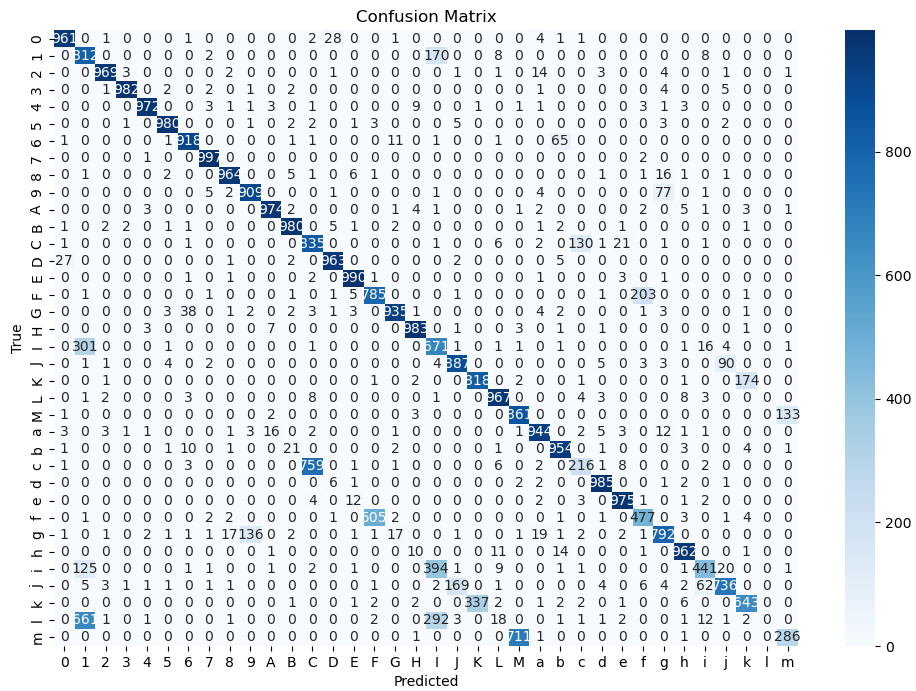
\includegraphics[width=0.9\linewidth]{Bilder/ConfusionMatrix/TrainTestFinal_cc2.png}
				\caption[Confusion Matrix des finalen experimentellen Modells - Ansatz 2]{Confusion Matrix - Finales experimentelles Modell - Ansatz 2}
				\label{fig:ConfusionMatrixTrainTestFinalcc2}
			\end{figure}
			
  
  
  \section{Fazit}
  
  \subsection{Abschließende Bewertung der Modelle}
  \textbf{Übersicht zur Leistung der Finalen Modelle auf den Testdaten}
    \begin{table}[h!]
  	\centering
  	\begin{tabular}{|l|c|c|c|}
  		\hline
  		\rowcolor{lightgray} \textbf{Metrik} & \textbf{Ausgangsmodell} & \textbf{Experim. Ansatz 1} &\textbf{Experim. Ansatz 2} \\ \hline
  		Top-1-Accuracy & 83,4\,\%  & 83,0\,\% & 82,0\,\% \\ \hline
  		Top-3-Accuracy & 98,7\,\%  & 84,2\,\% & 83,8\,\% \\ \hline
  		Top-5-Accuracy & 99,6\,\%  & 84,5\,\% & 84,0\,\% \\ \hline
  	\end{tabular}
  	\caption{Finale Ergebnisse aller Modelle}
  \end{table}
  
  \textbf{Übersicht zur Leistung der Finalen Modelle auf den Validierungsdaten}
      \begin{table}[h!]
  	\centering
  	\begin{tabular}{|l|c|c|c|}
  		\hline
  		\rowcolor{lightgray} \textbf{Metrik} & \textbf{Ausgangsmodell} & \textbf{Experim. Ansatz 1} &\textbf{Experim. Ansatz 2} \\ \hline
  		Top-1-Accuracy & 83,4\,\% & 82,8\,\% & 85,9\,\% \\ \hline
  		Top-3-Accuracy & 98,7\,\%  & 85,2\,\% & 87,5\,\% \\ \hline
  		Top-5-Accuracy & 99,6\,\%  & 85,6\,\% & 87,7\,\%  \\ \hline
  		Avg-Loss pro Bild & 0,717 & 2,97 & 2,81 \\ \hline
  	\end{tabular}
  	\caption{Finale Ergebnisse aller Modelle}
  \end{table}
  
  
	Es ist deutlich zu sehen, dass die Modelle mit den Experimentellen Ansatz die Leistung nicht übertreffen und zu schlechteren Vorhersagen neigen. Auch die abfallende Top-3 und Top-5 Accuracy kann als großes Problem angesehen werden.
	
	\textbf{Vorerst sollte man beim ursprünglichen Modell bleiben, da dieses die besten Ergebnisse liefert} und falls eine falsche Klasse vorhergesagt wurde, die richtige Klasse immer noch in den Top-3 Vorhersagen des Modells liegt. Auch aufgrund der hohen Top-3 Accuracy hat das Ausgangsmodell den kleinsten Durchschnittlichen Loss pro Bild und somit die kleinste Varianz zwischen den Wahrscheinlichkeiten bzgl. der Klassen einer Vorhersage.
  
  Im Nachhinein würde ich behaupten, dass ein solch kleines Modell, wie ich im \textbf{Experimentellen Ansatz 1} vorgestellt habe, zur Klassifizierung von Ziffern, Klein- und Großbuchstaben nicht für diese Aufgabe gewachsen ist. Bei meinen Mitstudierenden hat es laut deren Aussagen besser funktioniert, obwohl die Modelle sich nur marginal unterscheiden. Wahrscheinlich wäre ein ähnlich großes Modell wie ResNet-18 dieser Aufgabe besser gewachsen gewesen und ein weiteres Experiment wert. Auch einen Faktor für die Multiplizierung zwischen den einzelnen Modellen mit einzufügen wäre noch einen Versuch wert gewesen. Aufgrund der mangelnden Zeit, konnten diese Experimente nicht durchgeführt werden. 
  
  Der \textbf{Experimentelle Ansatz 2} bringt ein ähnliches Ergebnis wie der Experimentelle Ansatz 1. Der Unterschied ist, dass hier nicht die Abhängigkeit von der Gewichtsinitialisierung der Convolutional Layer wie im Ansatz 2 besteht und bei mehreren Versuchen eine konstante Leistung erreicht wird. 
  
  \subsection{Persönliches Fazit}
  Zur Recherche wurden größtenteils die Sprachmodelle ChatGPT \cite{noauthor_chatgpt_nodate} und DeepSeek \cite{noauthor_deepseek_nodate} eingesetzt und so z.B. den Hyperparameter-Suchraum zu beginn schon ein wenig einzuschränken. 
  Aus meinem Praktikum habe ich gelernt eine Protokollierung wie TensorBoard mit einzubauen, obwohl dies nicht gefordert war. Eine gute Protokollierung der Ergebnisse ist für ein Industrieprojekt unerlässlich und wäre hier mit Sicherheit noch als ausbaufähig zu bewerten. 
  Durch das Projekt konnte ich selbstständig ein kleines Machine-Learning Modell planen und aufbauen um besser mit der Materie vertraut zu werden. Dadurch dass ich auf die Workstations der OTH angewiesen war, war es teilweise etwas mühselig die Modelle zu trainieren und die Dateien per Kommandozeile hin- und herzuschieben. Beim Training unterliefen mir einige Fehler und so musste ich mehrmals das Hyperparameter-Tuning und eine Auswertung der Ergebnisse durchführen, dass mir letztendlich sehr viel Zeit kostete. Im Gesamten habe ich zu Lange für das Projekt, u.a. auch durch meine eigenen Fehler gebraucht, konnte aber dennoch einiges für die Zukunft lernen. 

  
  \clearpage % - bei Bedarf diesen Seitenumbruch entfernen
  \section{Anhang}
  
  \subsection{Visualisierung der Augmentationen}
  \label{subsec:augmentation-visualization}
  \begin{figure}[h!]
  	\centering
  	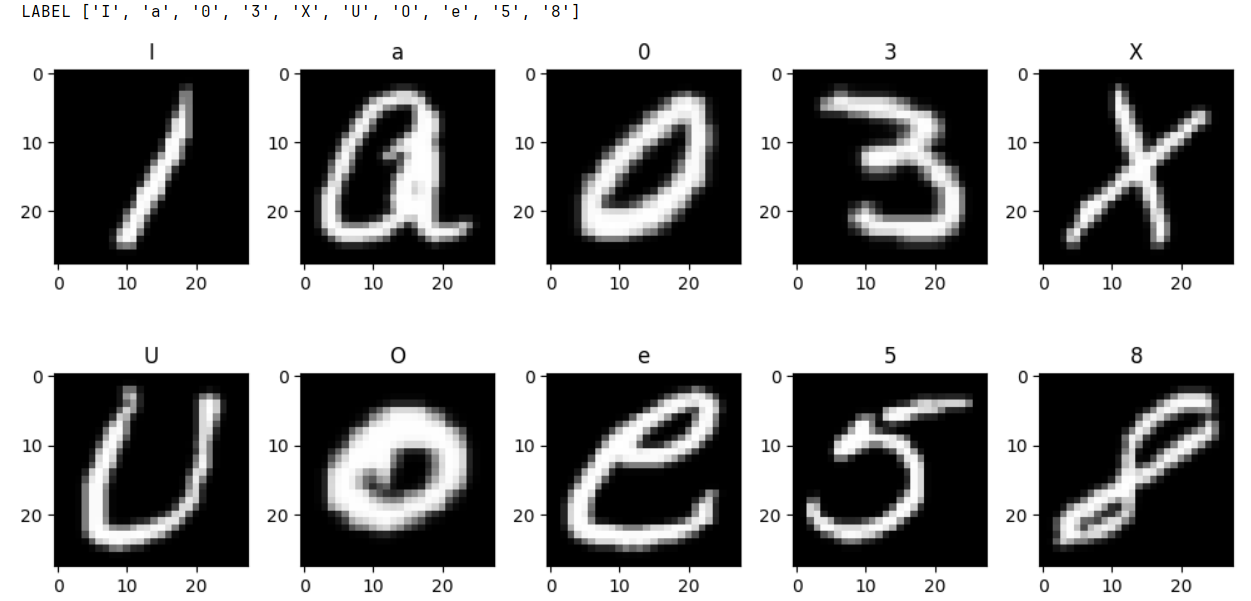
\includegraphics[width=0.7\linewidth]{Bilder/Augmentation_No.png}
  	\caption[GaussianBlur]{Original Bilder}
  	\label{fig:Augmentation_No}
  \end{figure}
  
  \begin{figure}[h!]
  	\centering
  	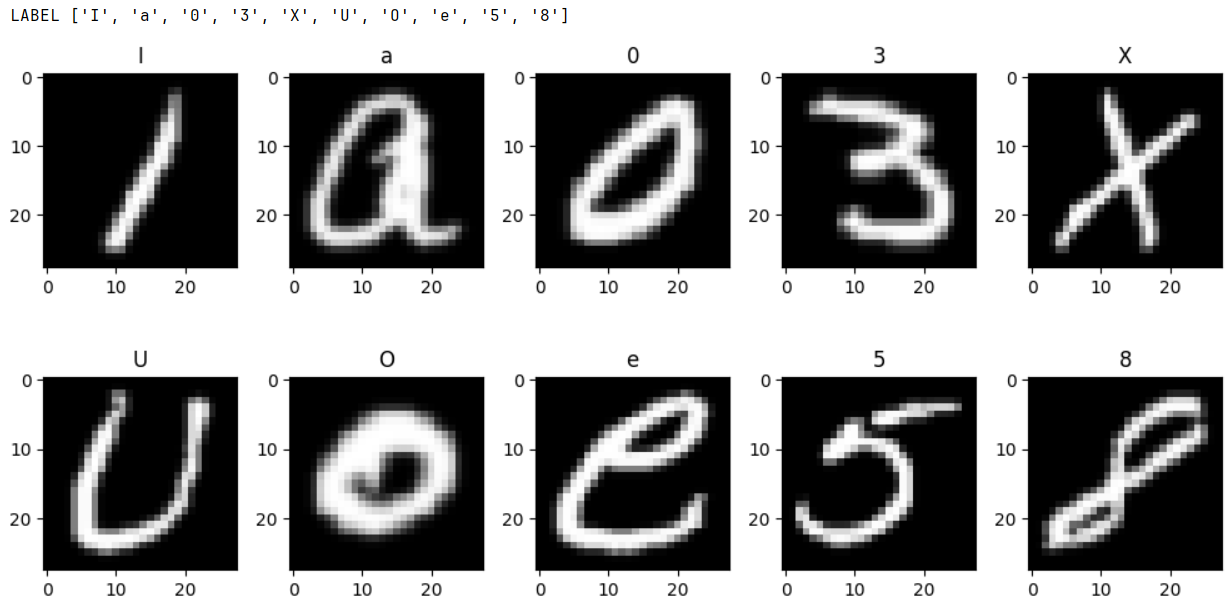
\includegraphics[width=0.7\linewidth]{Bilder/Augmentation_GuassianBlur.png}
  	\caption[Anwendung der Augmentation GuassianBlur]{Anwendung der Augmentation GuassianBlur}
  	\label{fig:Augment_GuassianBlur}
  \end{figure}
  
    \begin{figure}[h!]
  	\centering
  	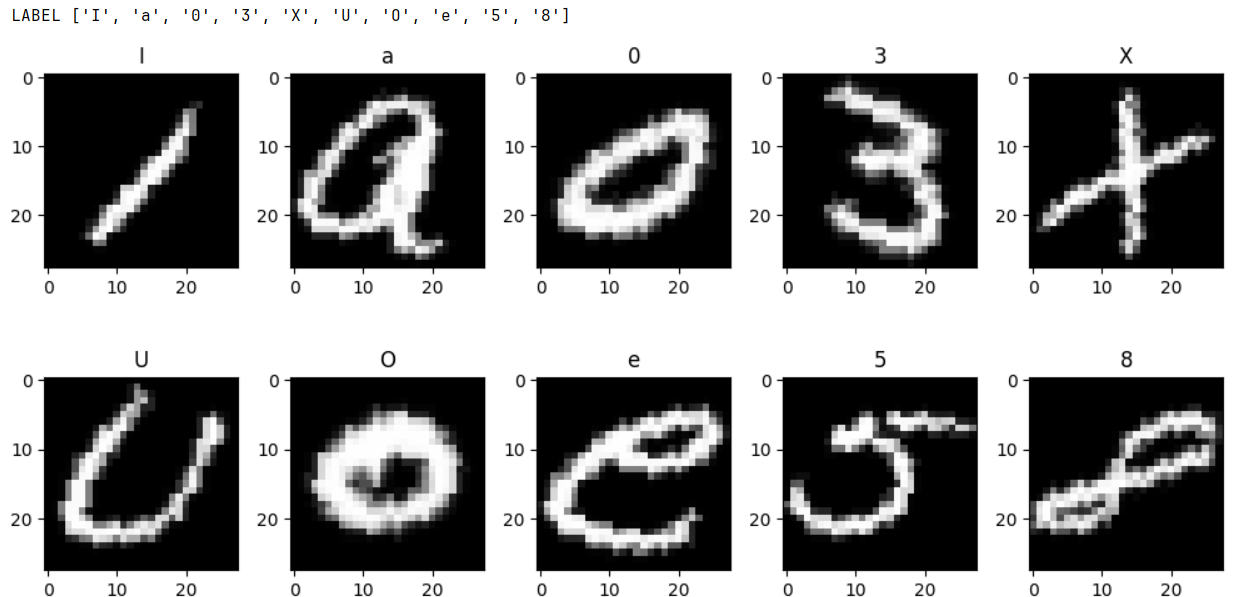
\includegraphics[width=0.7\linewidth]{Bilder/Augmentation_Rotation_15.png}
  	\caption[Anwendung der Augmentation Rotation 15°]{Anwendung der Augmentation Rotation 15°}
  	\label{fig:Augment_Rotation}
  \end{figure}
  
  \begin{figure}[h!]
  	\centering
  	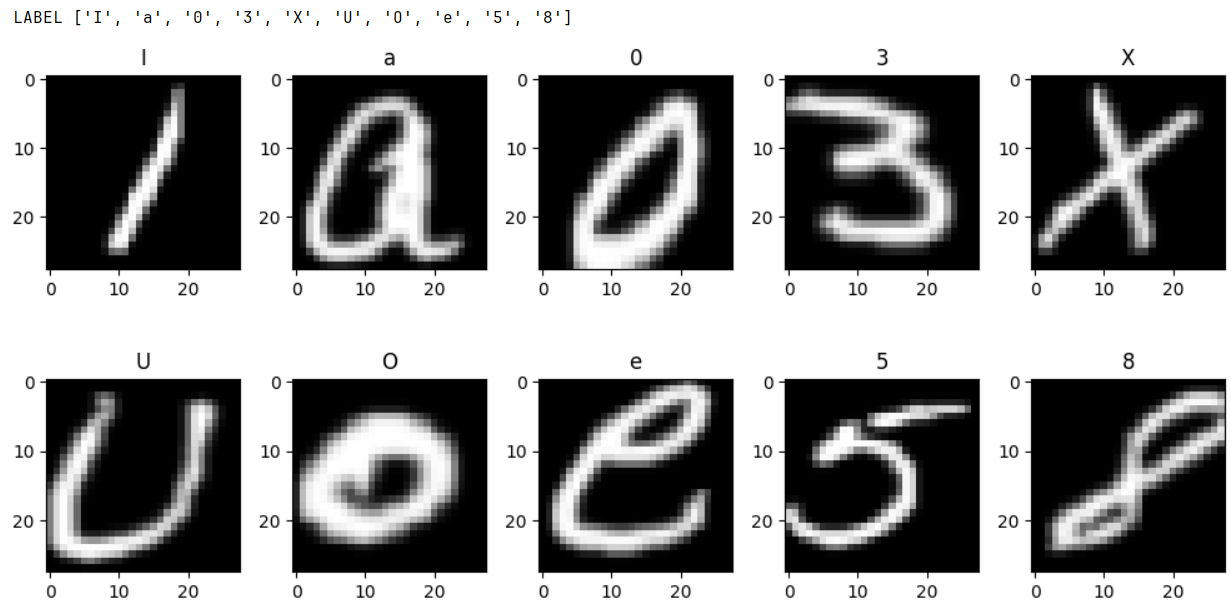
\includegraphics[width=0.7\linewidth]{Bilder/Augmentation_RandomResizedCrop.png}
  	\caption[Anwendung der Augmentation RandomResizedCrop]{Anwendung der Augmentation RandomResizedCrop}
  	\label{fig:Augment_RandomResizedCrop}
  \end{figure}
  

  \clearpage % - bei Bedarf diesen Seitenumbruch entfernen
  \subsection{Bedeutung der Hyperparameter}
  \begin{table}[h!]
  	\centering
  	\begin{tabular}{|p{0.3\linewidth}|>{\raggedright\arraybackslash}m{0.65\linewidth}|}
  		\hline
  		\rowcolor{lightgray} \multicolumn{1}{|c|}{\textbf{Parameter}} & \multicolumn{1}{c|}{\textbf{Bedeutung}} \\
  		\hline
  		\verb|only_train_classifier| & Ob nur mein Klassifizierer, der die 36-Zeichenklassen vorhersagt, trainiert werden soll (und der erste Convolutional Layer, der für die Bildgröße auf 28x28 Pixel angepasst wurde) \\ 
  		\hline
  		\verb|num_epochs| & Anzahl von Trainings-Epochen. Eine Epoche entspricht einem kompletten Durchlauf des aussortierten EMNIST-Datensatzes \\ 
  		\hline
  		\verb|batch_size| & Anzahl an Bildern, die pro Batch bzgl. eines Gradienten-Updates verarbeitet werden \\ 
  		\hline
  		\verb|probabilities| & Mit welcher Wahrscheinlichkeit werden die definierten Augmentierungen auf den Trainings- und Validierungsdatensatz angewendet? \\ 
  		\hline
  		\multicolumn{2}{|l|}{\small\rule{0pt}{1.5em}\textbf{AdamW-Optimizer}} \\ 
  		\hline
  		\verb|lr| & Initiale Lernrate / Schrittweite des Gradientenabstiegs des Modells \\ 
  		\hline
  		\verb|weight_decay| & L2-Regularisierungsterm im AdamW-Optimizer: Bestraft große Gewichte, um Overfitting zu reduzieren \\ 
  		\hline
  		\multicolumn{2}{|l|}{\small\rule{0pt}{1.5em}\textbf{ReduceLROnPlateau-Scheduler}} \\ 
  		\hline
  		\verb|sched_patience| & Anzahl der Epochen, wie lange keine Verbesserung der Top-1-Accuracy stattfinden darf, bevor die Lernrate des Modells gesenkt wird \\ \hline
  		\verb|sched_factor| & Faktor, mit dem die LR multipliziert wird, wenn die Lernrate verringert werden soll \\ 
  		\hline
  		\verb|sched_min_lr| & Die minimal mögliche Lernrate des Modells \\ 
  		\hline
  		\multicolumn{2}{|l|}{\small\rule{0pt}{1.5em}\textbf{Experimenteller Klassifierer}} \\ 
  		\hline
  		\texttt{train\_with\_\allowbreak CombinedClassifier} & Ob der Experimentelle Klassifizierer verwendet werden soll \\ 
  		\hline
  		\texttt{config\_\allowbreak CombinedClassifier} & Modellparameter des Experimentellen Klassifizierers \\ 
  		\hline
  	\end{tabular}
  	\caption{Bedeutung der Hyperparameter}
  	\label{tab:BedeutungHyperparameter}
  \end{table}
  
  
  
  
  
  \clearpage % - bei Bedarf diesen Seitenumbruch entfernen
  
  %
  % Literatur 
  %

  \phantomsection
  \addcontentsline{toc}{section}{Literatur}
  \bibliographystyle{natdin}
  \bibliography{ML2}
  

%\include{anhang} % zum Beispiel hier die ChatGPT-Chatprotokolle einbinden (oder als extra-Datei)

%C++-Code Microcontroller:
 %\lstinputlisting[lastline=92, language=C++]{../esp32/MicroController/MicroController.ino}

  %Ihr Code muss hier nicht vollständig wiedergegeben werden, aber evtl. interessante Ausschnitte.


%################### Ende ########################  
%  Die Literatur (für den nächsten Abschnitt) tragen Sie in die Datei \texttt{quellen.bib} ein. Diese Datei hat die BiB\TeX-Syntax (vgl. \url{https://ctan.org/pkg/bibtex}; BiB\TeX\ ist bei \href{https://www.heise.de/download/product/texstudio-62955}{\TeX studio} bzw. \href{https://www.overleaf.com}{Overleaf} dabei).
%  
%  Zur Literaturverwaltung verwenden Sie am besten Zotero \cite{zotero} oder JabRef \cite{jabref}. 
%  
%  Bei meiner \LaTeX-Installation ist der \texttt{natdin}-Style leider etwas buggy (bei \texttt{@book} wird die DOI-URL doppelt generiert, dafür fehlt sie bei \texttt{@inproceedings}). Allerdings funktioniert das
%  Attribut \texttt{lastchecked} für Webseiten (Publikationstyp \texttt{@misc}).


%  
%  Doku s. \url{https://ctan.org/pkg/listings}
%
%  Mit \verb|\lstinputlisting[lastline=14,language=C++]{MicroController.ino}| können auch (Ausschnitte von) 
%  externen Quellcode-Dateien eingebunden werden, so dass \emph{copy \& paste} von Quellcode
%  überflüssig wird.
%
%  
%  Bitte passen Sie in der \LaTeX-Datei \texttt{projektarbeit.tex} am Anfang folgende 
%  Zeilen an:
%  
%\begin{lstlisting}{language=[LaTeX]TeX}
%\newcommand*{\IhrVornameEins}{Erika}
%\end{lstlisting}
%  
%
%  Bei \href{https://www.heise.de/download/blog/Einfuehrung-in-LaTeX-3599742}{Heise (dies ist ein link)} 

\end{document}
